\chapter{Preliminaries} \label{sec:preliminaries}

\begin{table}[t]
\centering
\caption{
    Notation used in this paper.
    \label{tab:notation}
}
% \resizebox{\columnwidth}{!}{
\small
    \begin{tabular}{>{\centering\arraybackslash}m{2.1cm}|p{6cm}}
        \hline
        \textbf{Notation}           & \textbf{Description} \\ \hline
        $\mathcal{V}$               & The set of nodes in a graph                   \\ \hline
        $\mathcal{A}$               & The set of node types                         \\ \hline
        $\mathcal{E}$               & The set of edges in a graph                   \\ \hline
        $\mathcal{R}$               & The set of edge types/relations               \\ \hline
        $\mathcal{T}$               & The set of timestamps in a graph              \\ \hline
        $\mathcal{X}_{\phi(\cdot)}$ & Feature matrix for node type $\phi(\cdot)$    \\ \hline
        $\phi(v) \in \mathcal{A}$   & Type of node $v$                              \\ \hline
        $\psi(e) \in \mathcal{R}$   & Type of edge $e$                              \\ \hline
        $G_v$                       & $k$-hop neighborhood subgraph for node $v$    \\ \hline
        $d \in \mathbb{N}$          & Size of node embedding vector                 \\ \hline
        $E_v \in \mathbb{R}^d$      & Auxiliary embedding vector for node $v$       \\ \hline
        $Z_v \in \mathbb{R}^d$      & Primary embedding vector for node $v$         \\ \hline
        $Z_v^{\mathcal{E}}, Z_v^{\mathcal{T}} \in \mathbb{R}^d$ & Task specific embedding vectors for node $v$         \\ \hline
        $K \in \mathbb{N}$                                      & Number of communities                         \\ \hline
        $\mathcal{N}(\mu_k, \boldsymbol{\Sigma}_k), \theta_k$   & Parameters for the $k$'th cluster/community   \\ \hline
        ${\mu_k} \in \mathbb{R}^d$                              & $k$'th cluster mean vector                    \\ \hline
        $\boldsymbol{\Sigma}_k \in \mathbb{R}^{d\times d}$      & $k$'th cluster covariance vector              \\ \hline
        $\mathbf{z} \in \{0, .., K\}^{|\mathcal{V}|}$   & Community membership assignment vector        \\ \hline
        $\omega$                    & Interval window for temporal context sampling                     \\ \hline
        $P_l \in \mathcal{V}^l$     & Sampled context window of length $l$                              \\ \hline
        %                  &                      \\ \hline
    \end{tabular}
% }
\end{table}

We present a brief overview of the key concepts and notations used in community detection and graph representation learning. The notations can be found in \cref{tab:notation}. 

\begin{secDefinition}[\textbf{Heterogeneous graph}]
A heterogeneous graph, denoted as $G = (\mathcal{V}, \mathcal{E}, \mathcal{A}, \mathcal{R})$ consists of a set of nodes $\mathcal{V}$, a set of edges $\mathcal{E}$, and their associated type mapping functions $\phi : \mathcal{V} \rightarrow \mathcal{A}$ and $\psi : \mathcal{E} \rightarrow \mathcal{R}$. $\phi$ (resp. $\psi$) maps a node (resp. edge) to its type. $\mathcal{A}$ and $\mathcal{R}$ denote predefined sets of node and edge types, respectively, where $|\mathcal{A}| \geq 1$ and $|\mathcal{R}| \geq 1$. $G$ is a homogeneous graph if $|\mathcal{A}| = 1$ and $|\mathcal{R}| = 1$.
\end{secDefinition}

\noindent We define a multimodal information network by combining the notion of heterogeneous, continuous-time, and contentual networks. 
\begin{secDefinition}[\textbf{Multimodal graph}]
A multimodal graph is defined as $G = (\mathcal{V}, \mathcal{E}, \mathcal{A}, \mathcal{R}, \mathcal{T}, \mathcal{X})$ where $\mathcal{T}$ is a set of timestamps $t$ and $\mathcal{X}$ is a set of type specific feature matrices $\mathcal{X}_{\phi(\cdot)}$.
Each node $v \in \mathcal{V}$ (resp. edge $e \in \mathcal{E}$) has a time range $\tau(v) = [t_s, t_e]$  (resp. $\tau(e) = [t_s, t_e]$), indicating the time period on which it is considered valid, where $t_s, t_e \in \mathcal{T}$. 
In addition, each node $v$ has an attribute vector $\mathbf{x} \in \mathcal{X}_{\phi(v)}$.
\end{secDefinition}

\begin{secDefinition}[\textbf{Incompleteness constraints}] \label{def:incompleteness_constraints}
Real-world multimodal networks can be noisy, incomplete, and may change over time. 
In order to represent this information we introduce additional indicator functions to denote whether a node has a time interval $\mathbf{1}_{\mathcal{T}} : \mathcal{V} \rightarrow \{0, 1\}$, has a feature vector $\mathbf{1}_{\mathcal{X}} : \mathcal{V} \rightarrow \{0, 1\}$, or is unseen during training $\mathbf{1}_{\mathcal{V}} : \mathcal{V} \rightarrow \{0, 1\}$. 
We refer to the noisiness, incompleteness, and temporality as incompleteness constraints. 
\end{secDefinition}

\begin{secDefinition}[\textbf{Context window}]
A context window connects nodes based on some predefined criteria. Two nodes are \textit{context neighbors} if they occur in the same context window.
In our work, we use two different kinds of context windows. 
The first is the \textit{topological context window}. It connects two nodes $v_i$ and $v_j$ if there exists a k-hop path ${p}^{\mathcal{E}}_k$ in graph $G$ through which they are connected.
The second is \textit{temporal context window} ${p}^{\mathcal{T}}_{\omega}$. 
It connects $v_i$ and $v_j$ if they occur within a given time window $\omega = [t_s, t_e]$.
Going forward we use ${P}^{\mathcal{E}}_k$ and ${P}^{\mathcal{T}}_{\omega}$ to denote a fixed size sample of all possible context windows. 
\end{secDefinition}

\begin{secDefinition}[\textbf{Gaussian Mixture Model}]
% GMM
Gaussian mixture models (GMM) is a clustering algorithm that assumes the data points are generated by $K$ $d$-dimensional multivariate Gaussian distributions \cref{eq:gmm}.
Here cluster parameters $\theta_k$ for $k \in \{1, ..., K\}$ consist of the mean vector $\mu_k \in \mathbb{R}^d$ and the covariance matrix $\boldsymbol{\Sigma}_k \in \mathbb{R}^{d\times d}$.
A $K$-dimensional binary variable $\mathbf{z}$ is used to denote membership of a particular point $n$ where $\sum_k z_{nk} = 1$.
Mixing coefficients $\pi_k$ specify a marginal distribution over $\mathbf{z}$, such that $\sum_{n \in N} p(z_{nk} = 1) = \pi_k$ where $\pi_k \in [0, 1]$ and $\sum^K_{k=1} \pi_k = 1$.
Consequently $r_k$ represents conditional probability of $\mathbf{z}$ given a data point $\mathbf{x}$ \cref{eq:prob_assignment}. 

\begin{align}
p(\mathbf{x}; \theta) &= \sum^K_{k=1} \pi_k \mathcal{N}(\boldsymbol{\mu}_k, \boldsymbol{\Sigma}_k)\label{eq:gmm} \\
r_k = p(z_k = 1 | \mathbf{x}) &= \frac{
    \pi_{k} \mathcal{N}\left(\mathbf{x} \mid \boldsymbol{\mu}_{k}, \boldsymbol{\Sigma}_{k}\right)
}{
    \sum_{j=1}^{K} \pi_{j} \mathcal{N}\left(\mathbf{x} \mid \boldsymbol{\mu}_{j}, \boldsymbol{\Sigma}_{j}\right)
} \label{eq:prob_assignment}
\end{align}

% EM
Assuming that the points $\mathbf{X} \in \mathbb{R}^{N \times d}$ are drawn independently from the distribution, the log-likelihood function is given by \cref{eq:gmm_ll}.
The value of $\mu_k$, $\mathbf{\Sigma}_k$, $\pi_k$ can be found by setting derivative of $\ln p(\mathbf{X} \mid \boldsymbol{\pi}, \boldsymbol{\mu}, \mathbf{\Sigma})$ to zero with respect to their values yielding closed form equations \cref{eq:gm_mu,eq:gm_cov,eq:gm_pi}.
$N_k$ represents the number of points assigned to cluster $k$.
While model parameters can be computed given values of $\mathbf{X}$ and $\mathbf{r}$ are known, it is important to note that $\mathbf{r}$ is dependent on the model parameters \cref{eq:prob_assignment}.
Expectation-Maximization (EM) is an elegant iterative technique devised to find such clustering parameters.
Given an initial cluster assignment that may be obtained using k-means or a similar technique, \textit{expectation} (E) and \textit{maximization} (M) steps are applied alternatively \cref{fig:em}.
The E step uses current cluster parameters to evaluate posterior probabilities \cref{eq:prob_assignment}, while the M step uses these probabilities to compute new model parameters using \cref{eq:gm_mu,eq:gm_cov,eq:gm_pi}.
The model is deemed converged once the change in parameters or assignment falls below a certain threshold.

\begin{align}
\ln p(\mathbf{X} \mid \boldsymbol{\pi}, \boldsymbol{\mu}, \mathbf{\Sigma}) &= \sum_{n=1}^{N} \ln \left\{\sum_{k=1}^{K} \pi_{k} \mathcal{N}\left(\mathbf{x}_{n} \mid \boldsymbol{\mu}_{k}, \boldsymbol{\Sigma}_{k}\right)\right\} \label{eq:gmm_ll} \\
\boldsymbol{\mu}_{k} &= \frac{1}{N_{k}} \sum_{n=1}^{N} r_{nk} \mathbf{x}_{n} \label{eq:gm_mu} \\
\boldsymbol{\Sigma}_{k} &=\frac{1}{N_{k}} \sum_{n=1}^{N} r_{nk} \left(\mathbf{x}_{n}-\boldsymbol{\mu}_{k}\right)\left(\mathbf{x}_{n}-\boldsymbol{\mu}_{k}\right)^{\mathrm{T}} \label{eq:gm_cov} \\
\pi_{k} &= \frac{N_{k}}{N} \label{eq:gm_pi}
\end{align}

\begin{figure}[t!]
\centering
\subfigure[]{
% 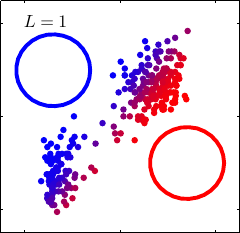
\includegraphics[width=0.40\columnwidth]{resources/em/EM1.png}
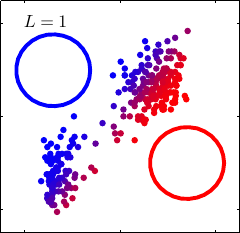
\includegraphics[width=0.21\textwidth]{resources/em/EM1.png}
}\quad
\subfigure[]{
% 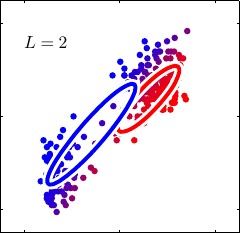
\includegraphics[width=0.40\columnwidth]{resources/em/EM2.png}
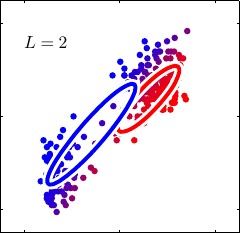
\includegraphics[width=0.21\textwidth]{resources/em/EM2.png}
}\quad
\subfigure[]{
% 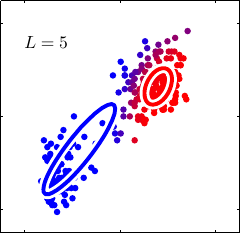
\includegraphics[width=0.40\columnwidth]{resources/em/EM3.png}
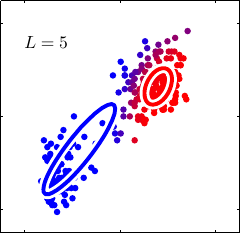
\includegraphics[width=0.21\textwidth]{resources/em/EM3.png}
}\quad
\subfigure[]{
% 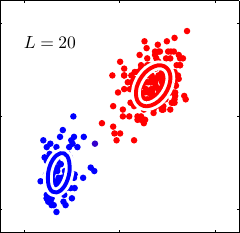
\includegraphics[width=0.40\columnwidth]{resources/em/EM4.png}
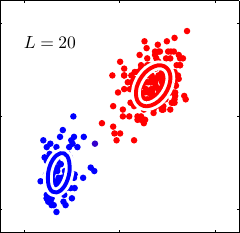
\includegraphics[width=0.21\textwidth]{resources/em/EM4.png}
}\quad
\caption{
Visualization of Expectation-Maximization algorithm \cite{bishopPatternRecognitionMachine2006}.
(a) Clusters are randomly initialized. 
(b) Cluster centers are updated according to the initial assignment (M step).
(c), (d) Expectation and Maximization steps are repeated until convergence.
}
\label{fig:em}
\end{figure}    

\end{secDefinition}

Gaussian Mixture Models suffer from severe overfitting problems in the form of single-point collapse and the fact that the number of clusters needs to be known a priori.
Bayesian parametric (BP) and non-parametric (BNP) mixture models aim to solve these issues by introducing prior distributions governing the model parameters ($\pi, \mu, \boldsymbol{\Sigma}$) and using maximum a priori (MAP) instead of maximum likelihood estimation. 

\begin{secDefinition}[\textbf{Dirichlet Process Mixture Model}] \label{sec:dpmm}
Dirichlet process mixture model (DPMM) is a part of BNP mixture models which finds a clustering solution when $K$ is unknown. 
DPMM extends GMM as it is an infinite mixture model \cref{eq:dpmm} with the Dirichlet process as prior distribution on the number of clusters \cref{eq:prior_dir}. 
Here hyperparameter $\alpha_0$ is the concentration parameter referring to the prior amount of observations associated with each component, and $\Gamma$ refers to the mathematical function "gamma" which in its essence is a generalization of the factorial function that can deal with any real number $>0$.
The cluster parameters $\theta$ are assumed to be i.i.d. and are drawn from a prior distribution. 
In our case, Normal Wishart Distribution (NW) \cref{eq:prior_nw} where hyperparameters $\kappa$ and $\nu$ represent the concentration parameter and degrees of freedom of the Wishart distribution respectively. 
The data is parameterized by the data mean $\mu$ and $\boldsymbol{\Lambda}$ which is the precision matrix (inverse of the covariance matrix $\boldsymbol{\Sigma}$).

\begin{align}
p(\boldsymbol{x}) &=\sum_{i=1}^{\infty} \pi_{i} \mathcal{N}\left(\boldsymbol{x}, \boldsymbol{\mu}_{i}, \boldsymbol{\Lambda}^{-1}\right) \label{eq:dpmm} \\
p(\boldsymbol{\pi}) &= \operatorname{Dir}\left(\boldsymbol{\pi}; \boldsymbol{\alpha}_{0}\right) = \frac{\Gamma(\alpha_0)}{\prod_{i=1}^{K} \Gamma(\alpha_0) } \prod_{i=1}^{K} \pi_{i}^{\alpha_{0}-1} \label{eq:prior_dir} \\
% C\left(\boldsymbol{\alpha}_{0}\right) \prod_{k=1}^{K} \pi_{k}^{\alpha_{0}-1} \label{eq:prior_dir} \\
p(\boldsymbol{\mu}, \boldsymbol{\Lambda}) &= \operatorname{NW}(\boldsymbol{\mu}, \boldsymbol{\Lambda}; \kappa_0, \mu_0, \nu_0, \boldsymbol{W}_0) \notag\\
&= \prod_{i=1}^{K} 
\underbrace{\mathcal{N}\left(\boldsymbol{\mu}_{i} \mid \mu_{0},\left(\kappa_{0} \boldsymbol{\Lambda}_{i}\right)^{-1}\right)}_{p(\mu_i | \boldsymbol{\Lambda}, \kappa_0, \mu_0)}
\underbrace{\mathcal{W}\left(\boldsymbol{\Lambda}_{i} \mid \mathbf{W}_{0}, \nu_{0}\right)}_{p(\boldsymbol{\Lambda}|\mathbf{W}_0, \nu_0)}
\label{eq:prior_nw}
\end{align}

The prior parameters $\alpha_0, \kappa_0$, and $\nu_0$ are set to a predetermined values, whereas prior parameters $\mu_0$ and $W_0$ are calculated on a sample of the full dataset using \cref{eq:nw_mu,eq:nw_W}. Here $\alpha_0, \nu_0,  \kappa_0 \in \mathbb{R}^+$ and $\nu_0 > d + 1$.

\begin{align}
\overline{\mathbf{x}}_{i} &=\frac{1}{N_{i}} \sum_{n=1}^{N} r_{n i} \mathbf{x}_{n} \label{eq:prior_comp_mu} \\
\mathbf{S}_{i} &=\frac{1}{N_{i}} \sum_{n=1}^{N} r_{n i}\left(\mathbf{x}_{n}-\overline{\mathbf{x}}_{i}\right)\left(\mathbf{x}_{n}-\overline{\mathbf{x}}_{i}\right)^{\mathrm{T}} \label{eq:prior_comp_cov}
\end{align}

EM can similarly be used to approximate solutions for DPM models. 
During the E step \cref{eq:prob_assignment} is once again used to estimate the assignments. 
While during the M step \cref{eq:prior_comp_mu,eq:prior_comp_cov} equations analogous to \cref{eq:gm_mu,eq:gm_cov} are used to estimate the data covariance and data mean.
Subsequently the following closed form equations are used to compute posterior parameters for the given prior \cref{eq:nw_kappa,eq:nw_mu,eq:nw_W,eq:nw_nu,eq:dir_pi}.
Given the posterior parameters, the new cluster parameters are inferred using \cref{eq:nw_mu,eq:nw_cov}.
When $\alpha_0$, $\kappa_0$, and $\nu_0$ are much smaller than $N$, the posterior distribution will be influenced primarily by the data rather than the prior.
We use $\lambda$ to denote computed posterior parameters.

\begin{align}
\pi_i &= \frac{N_i}{\sum_{k=1}^k N_i + \alpha_0} \label{eq:dir_pi} \\
\kappa_{i} &=\kappa_{0}+N_{i} \label{eq:nw_kappa} \\
\mu_{i} &=\frac{1}{\kappa_{i}}\left(\kappa_{0} \mu_{0}+N_{i} \overline{\mathbf{x}}_{i}\right) \label{eq:nw_mu} \\
\mathbf{W}_{i}^{-1} &=\mathbf{W}_{0}^{-1}+N_{i} \mathbf{S}_{i}+\frac{\kappa_{0} N_{i}}{\kappa_{0}+N_{i}}\left(\overline{\mathbf{x}}_{i}-\mu_{0}\right)\left(\overline{\mathbf{x}}_{i}-\mu_{0}\right)^{\mathrm{T}} \label{eq:nw_W} \\
\nu_{i} &=\nu_{0}+N_{i} \label{eq:nw_nu} \\
\boldsymbol{\Sigma}_i &= \frac{\nu \mathbf{W}_{i}^{-1}}{\nu - d + 1} \label{eq:nw_cov}
\end{align}

The described implementation solves overfitting and cluster count, though it is an incomplete one since in practice the cluster count has a defined upperbound $K$ (computationally and storage-wise).
While the clusters can get pushed out of existence, no additional clusters can be created.
To solve this issue many variants of DPMM have been proposed utilizing the Chinese Restaurant process, Collapsed Weight sampling, etc. 
We focus on the split/merge sampling algorithm introduced by Chang and Fisher III (DPMMSC) \cite{changParallelSamplingDP2013a}.
For an exhaustive discussion, we refer interested readers to \cite{bishopPatternRecognitionMachine2006, changSamplingComputerVision}.

DPMMSC exploits an alternate perspective in which DPMM is defined as a Monte Carlo Markov Chain if all the chosen priors are conjugate (i.e. prior distribution is in the same form as the posterior distribution).
The stationary distribution is defined by the probability of cluster parameters given the data observations \cref{eq:nw_stationary}.
Intuitively in this approach sampling methods are used to approximate the E step of EM by sampling from the current estimate of posterior distribution $p(\mathbf{z}|\mathbf{X}, \theta^{\text{old}})$ (proposal distribution), where during M step the new state $\theta$ is found.
A similar methodology is employed to transition between different values of $K$ by proposing $\theta$ directly.
As proposal space is unmanageably large, a greedy strategy is employed to propose the most promising states.

\begin{align}
    H_s &= \frac{
    \alpha \Gamma (N_{i_1}) p(X_{i_1}; \lambda_{i_1}) \Gamma (N_{i_2}) p(X_{i_2}; \lambda_{i_2})}{
    \Gamma (N_i) p(X_{i}; \lambda_i)} \label{eq:hastings_sratio}\\
    p(\mu_i, \boldsymbol{\Sigma}_i | \mathbf{X}_i) &= \operatorname{NW}(\boldsymbol{\mu}, \boldsymbol{\Lambda}; \kappa_0, \mu_0, \nu_0, \boldsymbol{W}_0) \label{eq:nw_stationary} \\
    p(\mathbf{X}; \lambda) &= \int p\left(\mathbf{X} \mid \boldsymbol{\mu}_{i}, \boldsymbol{\Sigma}_{i}\right) p\left(\boldsymbol{\mu}_{i}, \boldsymbol{\Sigma}_{i} ; \lambda\right) d\left(\boldsymbol{\mu}_{i}, \boldsymbol{\Sigma}_{i}\right) \notag \\
    &=\frac{1}{\pi^{\frac{N d}{2}}} 
    \frac{\Gamma_{d}\left(\nu_0 / 2\right)}{\Gamma_{d}(\nu_i / 2)} 
    \frac{|\nu_0 \boldsymbol{\Lambda}_0|^{\nu_0 / 2}}{\left|\nu_i \boldsymbol{\Lambda}_{i}\right|^{\nu_i / 2}}\left(\frac{\kappa_i}{\kappa_0}\right)^{d / 2} \label{eq:data_prob}
\end{align}

For each supercluster $i$, two auxiliary subclusters are defined with parameters $\theta_{i_1}$ and $\theta_{i_2}$ forming a two-component GMM.
Once subclusters are in a converged state, the split proposals are made given the supercluster and its two subcomponents.
Similarly, supercluster merges are proposed by picking $k$ nearest candidates for each supercluster.

The proposed candidates are either accepted or rejected by the Metropolis-Hastings (MH) algorithm moving the model to the next state.
As the split acceptance ratio $H_s$ is defined by the probability of data being sampled from the split state in contrast to the current state \cref{eq:hastings_sratio}.
Analogously, the merge ratio is its inverse, namely $\frac{1}{H_s}$.
\cref{eq:gmm_ll,eq:dir_pi,eq:prior_nw,eq:nw_stationary} are used to derive the marginal probability of data being generated by parameter set $\lambda$ given prior parameters \cref{eq:data_prob} (note that $\pi$ refers to the mathematical constant, and $\Gamma_d$ refers to mathematical function digamma).
%
The proposals are considered once the supercluster model has converged. If no proposal is accepted, then DPMMSC is considered as converged.
\end{secDefinition}

\begin{secDefinition}[\textbf{Graph Convolutional Neural Networks}]
Graph Convolutional Neural Networks (GCN) \cite{kipfSemiSupervisedClassificationGraph2017, hamiltonInductiveRepresentationLearning2017, kazemiRepresentationLearningDynamic2020} generate node embeddings given a spatial filter which is applied as a convolution given each node's graph neighborhood.
The convolution operation enables GCNs to propagate structural information of graphs throughout the network (referred to as message-passing). 
By layering this process, the receptive field of each node expands to its k-hop neighborhood.

Suppose $H_t^l$ is the representation of node $t$ at layer $l$, a forward step of the message-passing procedure is defined as \cref{eq:gnn_forward} where $N(t)$ is $t$'s neighboring node set and $\mathcal{E}(s, t)$ is the set of edges between nodes $t$ and its neighbor $s$. Here the operator $\operatorname{\textbf{Message}}(\cdot)$ extracts useful information from the neighboring source nodes $s$, while the $\operatorname{\textbf{Aggregate}}(\cdot)$ operator gathers the neighborhood information via some aggregation operator such as \textit{mean}, \textit{sum} or \textit{max} to get contextualized representation of $t$.

\begin{align}
    H_t^{(l)} = \underset{\forall s \in N(t), \forall e \in \mathcal{E}(s, t)}{\operatorname{\textbf{Aggregate}}} \left[\operatorname{\textbf{Message}}\left( H_s^{(l-1)}, e, H_t^{(l-1)} \right) \right] \label{eq:gnn_forward}
\end{align}

The time complexity to run a forward step over the entire training set is $O(|\mathcal{V}| \cdot deg \cdot d^2)$ where $deg$ refers to the average node degree.
While $deg \ll |\mathcal{V}|$ is true for most graphs, a vital optimization step is to sample a fixed size $N_v$ ensuring that $deg$ is bounded by a constant.
\end{secDefinition}

\begin{secDefinition}[\textbf{Heterogeneous Graph Transformer}]
\begin{figure}[!ht]
\centering
% 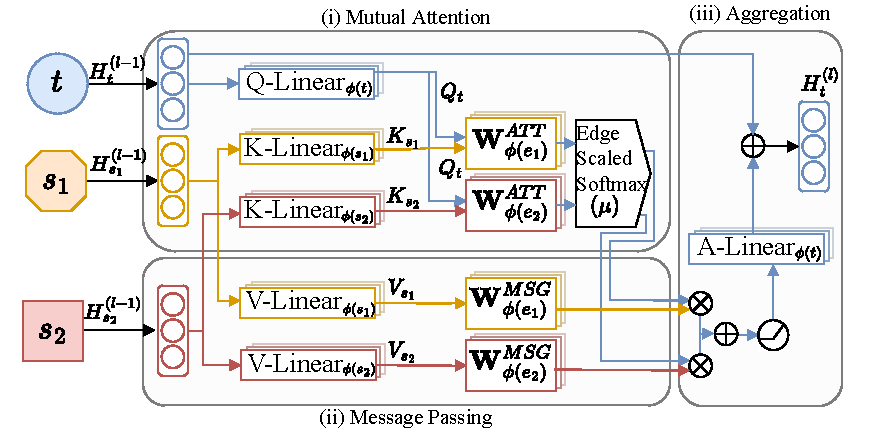
\includegraphics[width=\columnwidth]{resources/hgt.png}
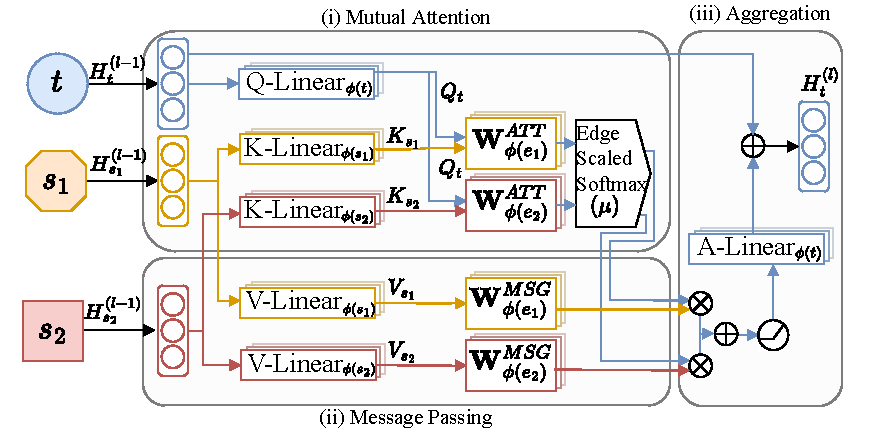
\includegraphics[width=0.8\columnwidth]{resources/hgt.pdf}
\caption{
    Visualization of a Heterogeneous Graph Transformer Layer. Given target node $t$ and neighboring source nodes $s_1$ and $s_2$ by edges $e_1$ and $e_2$, mutual attention and messages are computed. Within aggregation step the messages are attended and combined with previous target node embedding $H^{(l-1)}_t$ resulting in the new embedding vector $H^{(l)}_t$
}
\label{fig:hgt}
\end{figure}    

Classical GCNs focus mainly on homogeneous graphs. 
A fair amount of works describe ways to adapt existing algorithms by introducing a $\operatorname{\textbf{Message}}$ step parameterized by meta-topological types.
Based on the observation that the value of different connections varies given a node type, attention-based mechanisms are introduced into the aggregation process.
Inspired by success in NLP Heterogeneous Graph Transformer (HGT) \cite{huHeterogeneousGraphTransformer2020} adopts the transformer architecture \cite{vaswaniAttentionAllYou2017} by calculating mutual attention based on representation and meta-types of source, target and relation information.

\begin{align}
    H_t^l = \underset{\forall s \in N(t), \forall e \in \mathcal{E}(s, t)}{\operatorname{\textbf{Aggregate}}} \left[
    \operatorname{\textbf{Attention}}\left( s, e, t \right) \cdot
    \operatorname{\textbf{Message}}\left( s, e, t \right) 
    \right] \label{eq:hgt_forward}
\end{align}

HGT consists mainly of three components, (i) mutual attention possession performance of each source node, (ii) message passing extracts information from source nodes, and (iii) target-specific aggregation which combines the neighborhood messages.
A general form for a forward pass is defined as \cref{eq:hgt_forward} and is visualized in \cref{fig:hgt}.

The attention vector is calculated by mapping source node $s$ into Key $K$ and target node $t$ into a Query $Q$ vectors \cref{eq:hgt_K,eq:hgt_Q}.
A single head attention vector is calculated as inner product similarity vector between Key $K$ and Query $Q$ vectors (See \cref{eq:hgt_att_head}) given a relation specific interaction matrix, where prior tensor $\mu \in \mathbb{R}^{|\mathcal{A}| \times |\mathcal{R}| \times |\mathcal{A}|}$ denotes significance of each relation triplet. 
$K(s)$ and $Q(t)$ are computed as projections of source $s$ and target $t$ nodes respectively \cref{eq:hgt_K,eq:hgt_Q}.
The final attention vector results from a concatenation of $h$ attention heads per source node \cref{eq:hgt_att}.

\begin{align}
    \operatorname{\textbf{Attention}}_{H G T}(s, e, t) &= \underset{\forall s \in N(t)}{\operatorname{Softmax}} \left(\underset{i \in[1, h]}{\|} \operatorname{\textit{ATT-Head}}^{i}(s, e, t)\right) \label{eq:hgt_att} \\
        \operatorname{\mathit{ATT-Head}}^{i}(s, e, t) &=\left(K^{i}(s) W_{\psi(e)}^{A T T} Q^{i}(t)^{T}\right) \cdot \frac{\mu_{\langle\phi(s), \psi(e), \phi(t)\rangle}}{\sqrt{d}}  \label{eq:hgt_att_head} \\
        K^{i}(s) &=\operatorname{K-Linear}_{\phi(s)}^{i}\left(H^{(l-1)}_s\right) \label{eq:hgt_K} \\
        Q^{i}(t) &=\operatorname{Q-Linear}_{\phi(t)}^{i}\left(H^{(l-1)}_t\right) \label{eq:hgt_Q}
\end{align}

Similarly, the multi-head message is computed by applying type-dependent projection ($\operatorname{V-Linear}$) to the input source node representation and transforming it using the edge type matrix $W_{\psi(e)}^{MSG} \in \mathbb{R}^{\frac{d}{h} \times \frac{d}{h}}$ to incorporate the relation dependency into the result \cref{eq:hgt_msg_head}. 
In both operations, edge interaction matrices and the head-specific type projection matrices are shared to minimize the number of used parameters.  

\begin{align}
    \operatorname{\textbf{Message}}_{HGT}(s, e, t) &=\underset{i \in[1 \ldots h]}{\|} \operatorname{\textit{MSG-Head}}^{i}(s, e, t) \label{eq:hgt_msg} \\
        \operatorname{\mathit{MSG-Head}}^{i}(s, e, t) &=\operatorname{V-Linear}{ }_{\phi(s)}^{i}\left(H^{(l-1)}_s\right) W_{\psi(e)}^{MSG} \label{eq:hgt_msg_head}
\end{align}

Finally, during the aggregation step, the calculated attention is applied to neighborhood messages and summed into the neighborhood representation vector \cref{eq:hgt_neigh}.
The final node representation vector $H^{(l)}_t$ results from the summation of the projected neighborhood vector into the target node space and the previous representation of the target vector \cref{eq:hgt_agg}.

\begin{align}
    \widetilde{H}^{(l)}_t &=\underset{\forall s \in N(t)}{\oplus}\left(\operatorname { \textbf{Attention} }_{HGT}(s, e, t) \cdot \operatorname{\textbf{Message}}_{HGT}(s, e, t)\right) \label{eq:hgt_neigh} \\
    H^{(l)}_t &=\operatorname{A-Linear}_{\phi(t)}\left[\sigma\left(\widetilde{H}^{(l)}_t\right)\right]+H^{(l-1)}_t \label{eq:hgt_agg}
\end{align}

See \cref{fig:hgt} for a visualization of a forward pass of single layer HGT. 

\end{secDefinition}

\vspace{3mm}
\noindent\textbf{Problem formulation.} 
Given a multimodal graph $G$, our goal is to learn a node embedding function $\zeta: G_{v} \rightarrow \mathbb{R}^{d}$ which given a $k$-hop neighborhood subgraph $G_{v}$ of node $v$ produces a $d$-dimensional embedding vector $Z_v$.
%The embedding $Z_v$ should minimize the proximity to other nodes embeddings given they are topological and/or temporal context neighbors of node $v$.
The objective is to minimize the distance between embedding $Z_v$ to other node embeddings, given that they are topological and/or temporal context neighbors of node $v$.
Taking into account incompleteness constraints (\cref{def:incompleteness_constraints}), $\zeta$ should work under any valuation of $(\mathbf{1}_{\mathcal{X}(v)}, \mathbf{1}_{\mathcal{T}(v)}, \mathbf{1}_{\mathcal{V}(v)})$.
We also aim to find community parameters $\mathbf{\theta} = \{\mathcal{N}(\mu_1, \Sigma_1), ..., \mathcal{N}(\mu_K, \Sigma_K)\}$ and node-to-community assignment $\mathbf{z} \in \{0, .., K\}^{|\mathcal{V}|}$ such that their members have a low inter-proximity in contrast to other nodes.
Finally, the found community count $K$ should approximate the ground truth number of communities.